\section{Post-quantum cryptography (PQC)} \label{post-quantum-cryptography-pqc}

Despite offering in principle perfect security, there are several major issues with QKD as a form of cryptography that make it undesirable:
\begin{itemize}
	\item Quantum infrastructure is and likely always will be extremely expensive compared to our existing classical infrastructure.
	\item Globally we already have multi-trillion-dollar infrastructure for classical communication that cannot be made compatible with qubits.
	\item That quantum information cannot be broadcast essentially rules it out for mobile or roaming devices.
	\item It requires classical authentication of the public channel.
	\item Keys have one-time use, meaning quantum bandwidth must be extremely high.
	\item It does not facilitate public-key cryptography, only private-key cryptography.
	\item Our existing private-key cryptography is not vulnerable to any known quantum attacks beyond a Grover attack --- easily offset via longer key lengths --- and has the advantage of key reusability.
\end{itemize}

In light of these disadvantages, it would be far more attractive if \emph{classical} encryption techniques could be developed that are both quantum-proof and satisfy our need for public-key encryption and digital signatures. This has now become a major field of research.

If successful, this would imply that becoming cryptographically quantum-proof would become a trivial matter of substituting cryptographic software libraries and all our existing software would be safe. It doesn't take much convincing to see how much more desirable this would be than rolling out trillions of dollars in new infrastructure that only promises improved \emph{private}-key cryptography, which has limited utility in isolation.

\subsection{Hash-based digital signatures} \label{hash-based-digital-signatures}

Hash-based digital signatures are an alternative to RSA/ECC in which the security of signatures is inherited from the pre-image resistance of hash functions --- so long as we employ strong hash functions which are computationally hard to invert, the digital signature will also be secure.

\subsubsection{Lamport one-time signatures} \label{lamport-one-time-signatures}

\begin{figure*}[!htb]
\begin{tabular}{|l|l|l|l|l|}
\hline
\textbf{Bit} & \textbf{Private key} & \textbf{Public key} & \textbf{Message} & \textbf{Signature} \\
\hline
\hline
$1$ & ${\tt priv}_0(1),{\tt priv}_1(1)$ & ${\tt hash}({\tt priv}_0(1)),{\tt hash}({\tt priv}_1(1))$ & $m_1$ & ${\tt priv}_{m_1}(1)$ \\
$2$ & ${\tt priv}_0(2),{\tt priv}_1(2)$ & ${\tt hash}({\tt priv}_0(2)),{\tt hash}({\tt priv}_1(2))$ & $m_2$ & ${\tt priv}_{m_2}(2)$ \\
$3$ & ${\tt priv}_0(3),{\tt priv}_1(3)$ & ${\tt hash}({\tt priv}_0(3)),{\tt hash}({\tt priv}_1(3))$ & $m_3$ & ${\tt priv}_{m_3}(3)$ \\
$4$ & ${\tt priv}_0(4),{\tt priv}_1(4)$ & ${\tt hash}({\tt priv}_0(4)),{\tt hash}({\tt priv}_1(4))$ & $m_4$ & ${\tt priv}_{m_4}(4)$ \\
$5$ & ${\tt priv}_0(5),{\tt priv}_1(5)$ & ${\tt hash}({\tt priv}_0(5)),{\tt hash}({\tt priv}_1(5))$ & $m_5$ & ${\tt priv}_{m_5}(5)$ \\
$\vdots$ & $\vdots$ & $\vdots$ & $\vdots$ & $\vdots$ \\
$n$ & ${\tt priv}_0(n),{\tt priv}_1(n)$ & ${\tt hash}({\tt priv}_0(n)),{\tt hash}({\tt priv}_1(n))$ & $m_n$ & ${\tt priv}_{m_n}$($n$) \\
\hline
\end{tabular}
\caption{Signature scheme for the Lamport hash-based digital signature.} \label{fig:Lamport_sig}
\end{figure*}

The first hash-based digital signature scheme was the Lamport signature \cite{bib:lamport1979constructing}. While the Lamport signature is very strong it has the disadvantage that it is a \emph{one-time signature} --- it can only be used once. This makes it a not-so-useful signature scheme on its own. However, as we will see later, it can be used as a cryptographic primitive for the Merkle Signature Scheme which does allow reusable public keys.

Suppose we want to sign a 256-bit message digest (i.e a 256-bit hash of the full message we are signing). The private and public keys are established as follows:

\paragraph{Private key}

We choose 256 pairs of 256-bit random numbers. For the $i$th pair we denote these two numbers as ${\tt priv}_m(i)$ where $m=\{0,1\}$ index the two numbers in the pair. This has a total memory footprint of 128Kb.

\paragraph{Public key}

The associated public key is the correspondingly indexed set of 256-bit hashes of the private key numbers, such that,
\begin{align}
	{\tt pub}_m(i) = {\tt hash}({\tt priv}_m(i)).
\end{align}
This also has a total memory footprint of 128Kb. Thus the key pair is 256Kb in length.

Alice makes all the numbers comprising ${\tt pub}_m(i)$ public. Note that because of the pre-image resistance of the hash function, no one can determine any of the numbers comprising the private key from their respective publicly available hashes. Hence in this example, the \emph{trapdoor function} is a cryptographic hash function, which to the best of our understanding cannot be strongly compromised by quantum computers (see Grover's algorithm in Sec.~\ref{grovers-algorithm}).

\paragraph{Signing}

Our table of private and pubic keys corresponding to each bit in the message is shown in the table in Fig.~\ref{fig:Lamport_sig}. The signature of the message is made by making public the private keys for the corresponding message bits. That is, if the $n\mathrm{th}$ message bit is 0 we add ${\tt priv_0}(n)$ to the signature, and if it was 1 we add ${\tt priv_1}(n)$ to the signature. %The signature scheme is shown in Fig.~\ref{fig:Lamport_sig}.

Supposing the signature was shared \emph{after} the public key was made public, by selectively revealing the associated private key strings, their pre-image resistance implies they must have been known beforehand to whoever made the signature. ???? IS THIS TIMING ARGUMENT RIGHT

The reason the key is one-time is because each time it is used we reveal a part of the private key, thereby opening avenues for the associated bits to be fraudulently signed, and after a moderate number of reuses of the key-pair all private key strings will be known and any message can be fraudulently signed.

\subsubsection{Merkle Signature Scheme} \label{merkle-signature-scheme}

The Lamport signature is extremely secure, so long as the underlying hash function satisfies our cryptographic criteria, which to the best of our understanding contemporary hash functions like SHA-256 do. However, their one-time nature provides them with highly limited utility. What we really need is signatures that can be reused many times, like existing RSA and ECC schemes. To achieve this, using Lamport signatures as the basic building block, reusable signatures can be made by combining them with Merkle tree data structures.

Merkle trees are tree graphs where every node is labelled by the hash of its concatenated child node labels (see Fig.~\ref{fig:Merkle}), 
\begin{align}
	\mathtt{parent}=\mathtt{hash}(\mathtt{child}_1|\dots|\mathtt{child}_n).
\end{align}
This bestows the property that the labels of parent nodes can always be calculated if the labels of their child nodes are known, but not vice-versa owing to the hash function's pre-image resistance property.

\begin{figure}[!htb]
	\centering
	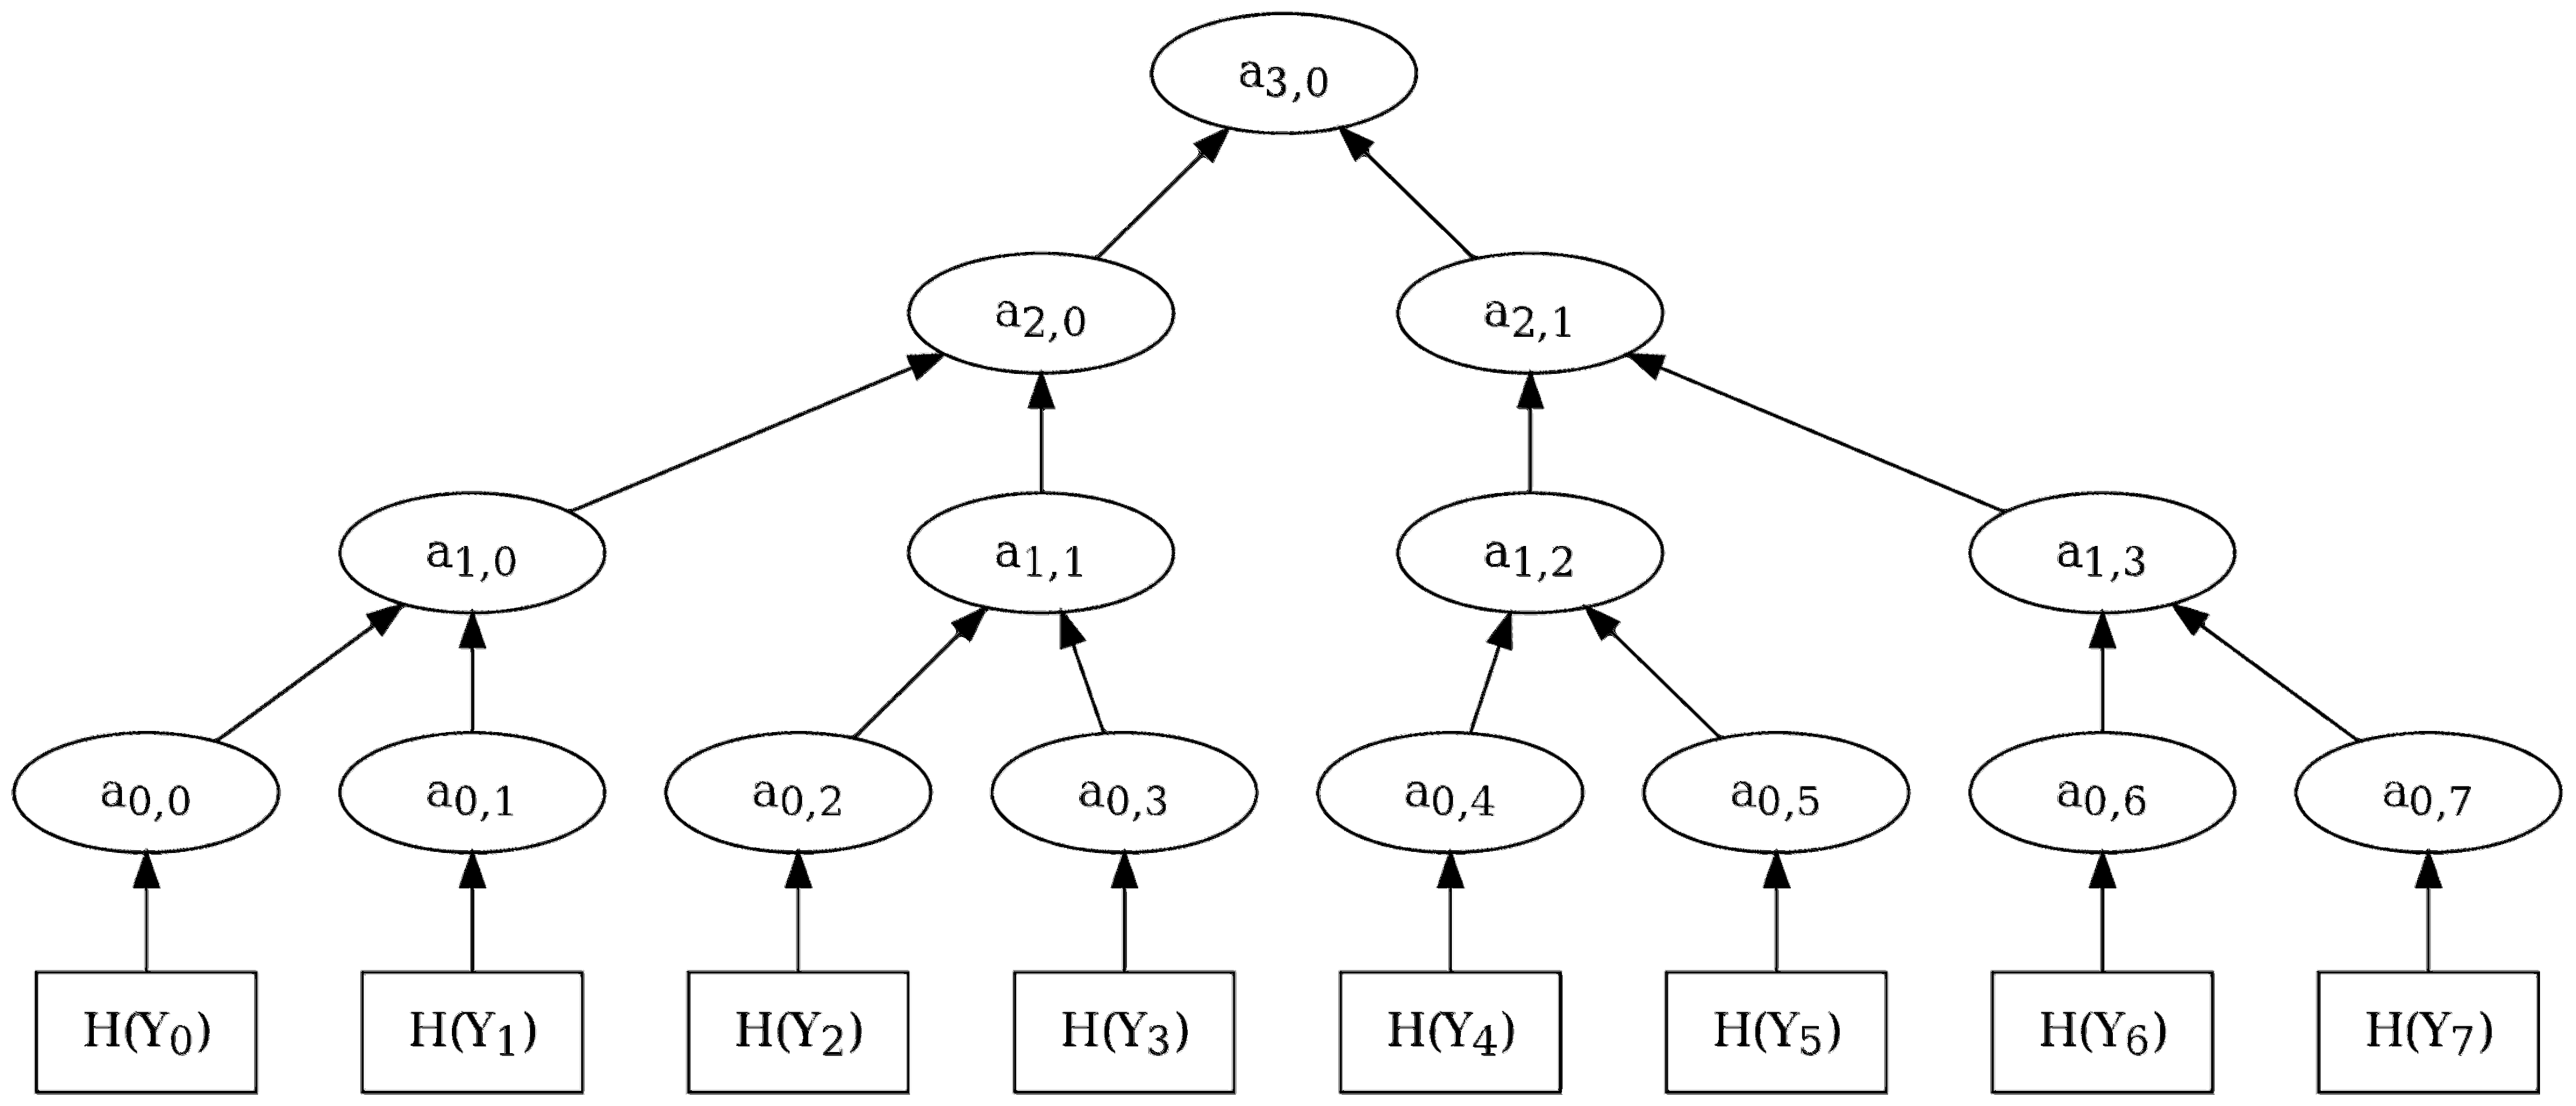
\includegraphics[width=\columnwidth]{figures/Merkle_tree}
	\caption{A Merkle tree data structure. Each node is labeled by the hash of the concatenated labels of its children. The pre-image resistance of the hash function implies that parent nodes can be calculated from their child nodes but not vice-versa. (Image from Wikipedia)} \label{fig:Merkle}
\end{figure}

In the \emph{Merkle signature scheme} we take a very large such Merkle tree, where all the leaf nodes are labelled by the public keys of individual one-time Lamport signatures. The reusable master public key is given by the label of the root node at the top of the tree.

We now want to have a mechanism that allows any of the leaf one-time signatures to demonstrably trace back to the master key. Clearly if all the leaf nodes are revealed we can easily do this. But we won't do that since that would carry an enormous memory footprint. We don't need to either, since the master key can be derived from any chain from a leaf node to the root node, provided the necessary child nodes along that path are selectively revealed. This is referred to as an \emph{authentication path}, as shown in Fig.~\ref{fig:auth_path}. Note that only a single leaf node (i.e one-time signature) need be revealed to form an authentication path to the root node.

\begin{figure}[!htb]
	\centering
	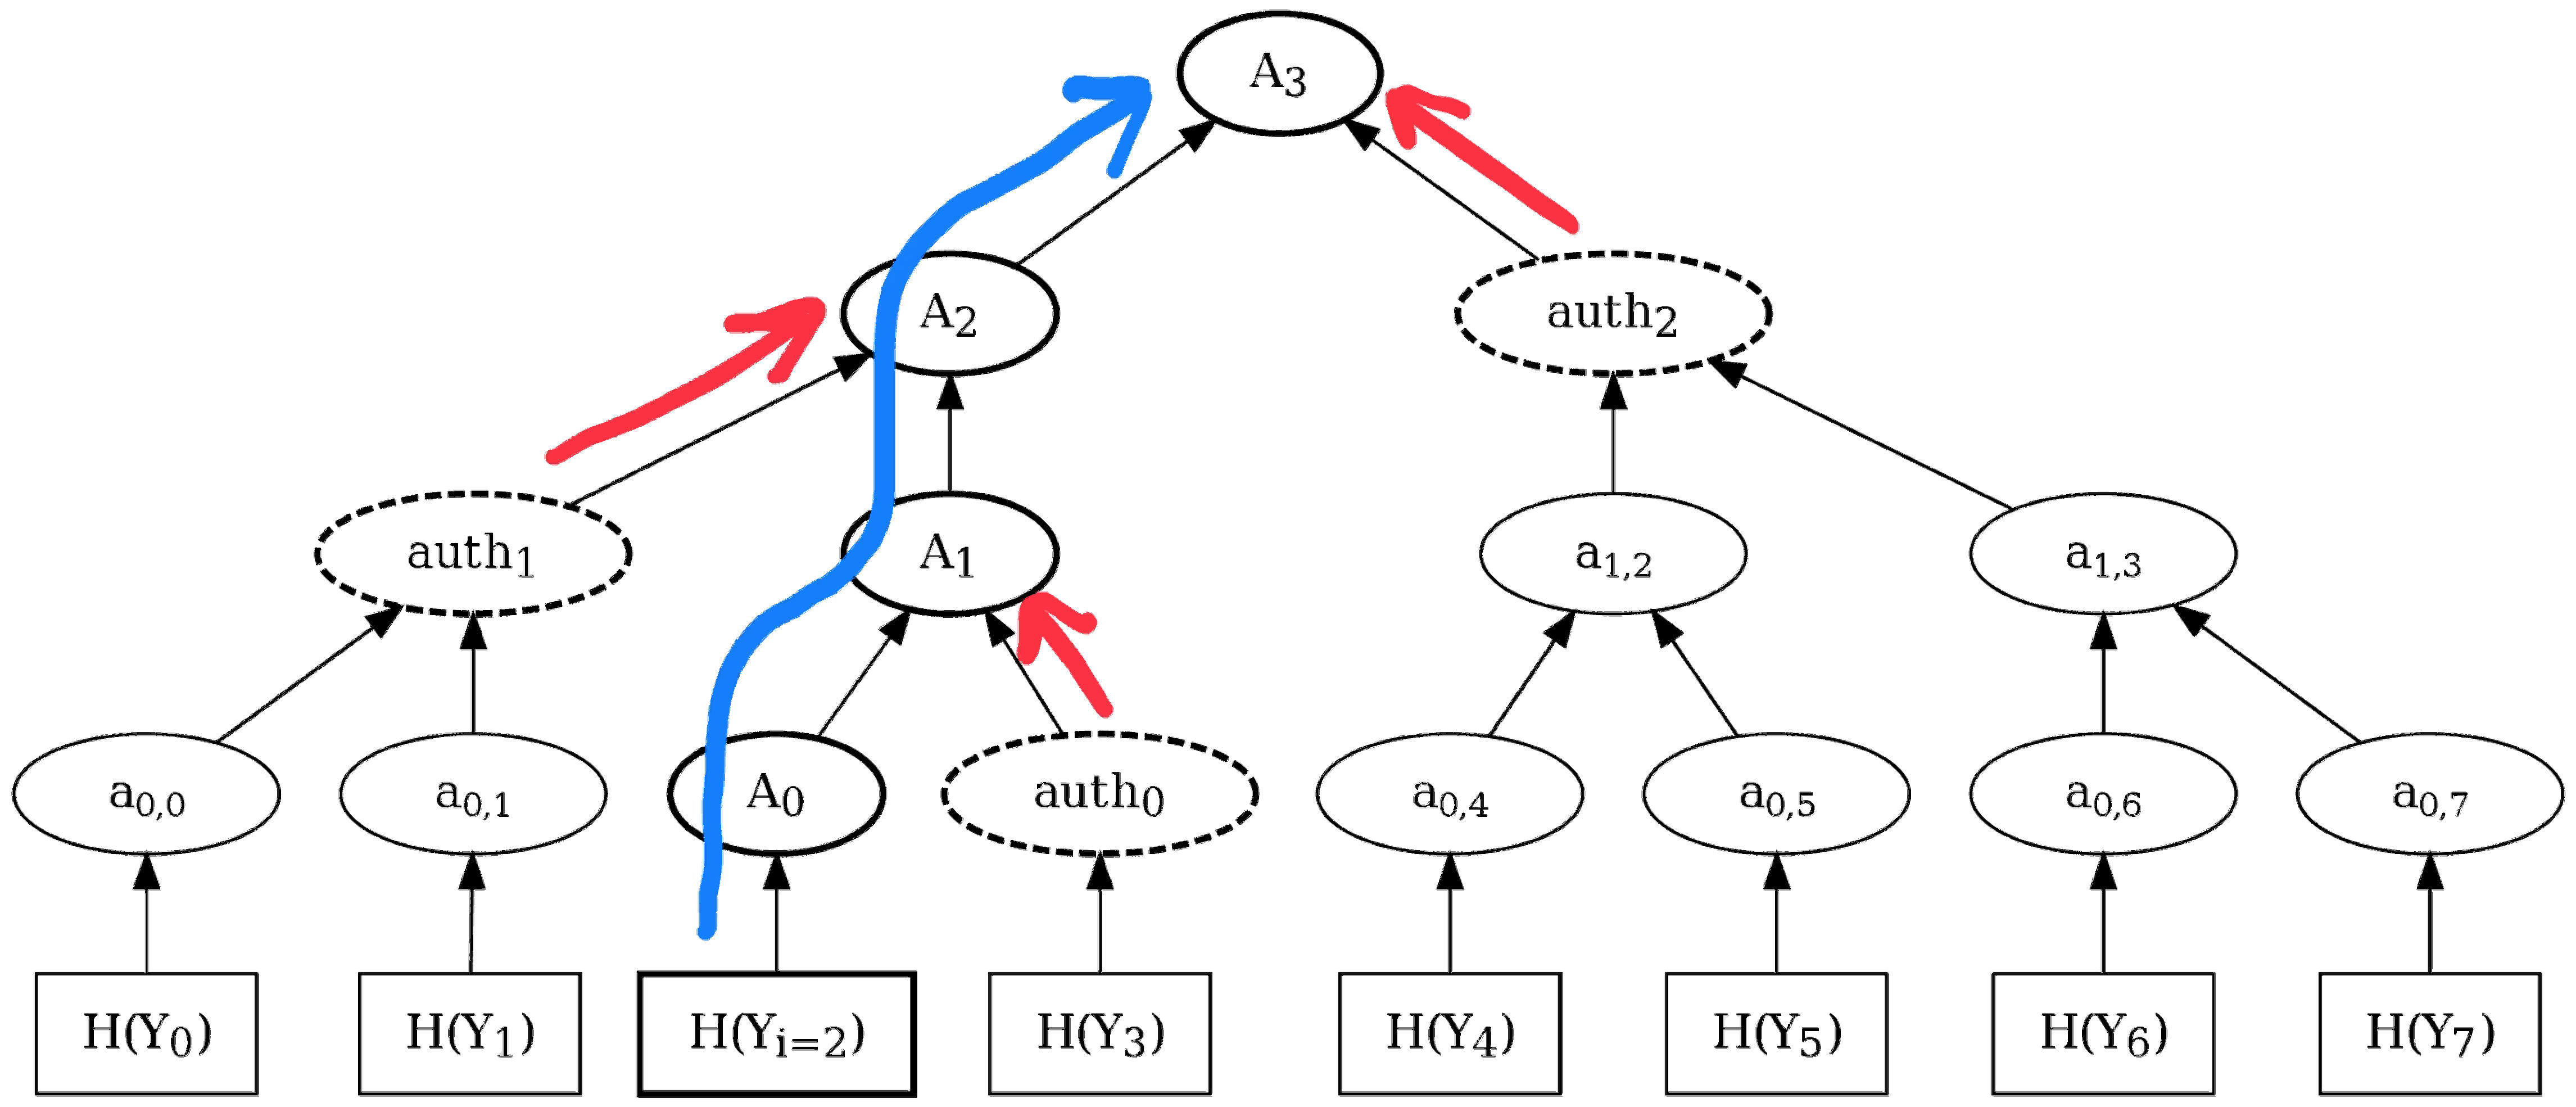
\includegraphics[width=\columnwidth]{figures/Authentication_path}
	\caption{Authentication path for leaf 2. The path to the master key is shown in blue. The additional information that must be revealed to authenticate that path is shown in red. None of the information in the authentication path reveals other leaf nodes based on the pre-image resistance of the hash function. (Image from Wikipedia)} \label{fig:auth_path}
\end{figure}

Since binary trees have depth logarithmic in their number of leaves, this means the size of the authentication chain which must be revealed in order to prove the legitimacy of a single leaf node has only logarithmic overhead in the reusability of the master key, a very efficient overhead. If we consider that $2^{32}\approx 4.3\times 10^9$, this means with a measly factor of 32 overhead in the size of our signatures we are able to have a master public key that can be reused 4.3 billion times. The caveat is that the entire Merkle tree with 4.3 billion key-pairs must be prepared in advance and held by the signatory.

Since the invention of the Merkle signature scheme, various other hash-based schemes have been developed also, such as the Extended Merkle Signature Scheme (XMSS) \cite{bib:XMSS}.

\subsection{Lattice-based cryptography} \label{lattice-based-cryptography}

In addition to the approach of hash-based digital signatures in which only symmetric-key cryptography is used, cryptographers have been looking into the possibility of constructing public-key cryptography based on the hardness of solving certain problems in high-dimensional lattices.  A lattice is a discrete subgroup in a euclidean space $\mathbb R^n$, or the set of all linear combinations of a basis for $\mathbb R^n$ with integer coefficients.  Like a euclidean space, a lattice can have many bases, some of which are ``nicer'' than others in the sense that certain problems are easier to solve in a nice basis.  For example, the problem of finding the shortest (nonzero) vector (SVP) is believed to be hard in a not-so-nice basis.  Furthermore, we do not know any quantum algorithms that have nontrivial speedup over the best classical algorithms for solving certain lattice problems, making these problems a good starting point for constructing PQC.

(??? Details on Kyber, Dilithium, and Falcon, the lattice-based PQC newly standardised by NIST. ???)

\subsection{Standardisation} \label{standardisation}

As with all the major cryptographic primitives we rely on today (e.g AES, SHA, RSA, ECC) they tend to only achieve widespread trust and adoption once they become standardised. Once standardisation takes place, software libraries implementing these primitives will emerge to substitute in for our existing ones and developers will have confidence in the ability for their cryptographic techniques to be interoperable with others.

Currently in the United States the National Institute of Standards \& Technology (NIST) is in the process of standardising post-quantum cryptography. This process will likely still take some time --- cryptography is a highly nuanced and complex field and standardisation sets a high bar for testing and verification. However once this process is complete, we can reasonably expect that post-quantum cryptography will become the norm and switching to post-quantum cryptography will be as simple as substituting software libraries.

Further details about NIST's post-quantum standardisation project can be found at \cite{bib:NIST_PQC}.

\subsection{Outlook}

Although the promise of PQC is quantum resistant public-key cryptography, this is something that is \emph{believed} rather than \emph{proven} to be the case, in the same way that RSA/ECC are believed to be robust against classical attacks but not proven to be so.

In the absence of formal mathematical proofs of their security, the real integrity test of PQC will be the test of time. We can have very high confidence that RSA/ECC are robust against classical attacks, simply because if anyone had found such an attack we would almost certainly know about it by virtue of us all having empty wallets. In effect there is an enormous cash prize for any hacker able to compromise RSA/ECC, and the failure of anyone to claim it implies a high level of confidence in their integrity.

Similarly, as PQC becomes standardised and sees widespread adoption our level of confidence in its integrity will be a function of the test of time as adversaries put it to the test using both classical and future quantum techniques. It would be a mistake to simply take for granted at the point of standardisation that PQC algorithms are as robust as advertised.